%%%%%%%%%%%%%%%%%%%%%%%%%%%%%%%%%%%%%%%%%
% Report Template
% LaTeX Template
% Version 1.2.1 (2024-02-20)
%
% This template was adapted by:
% Jonathan Decker (jonathan.decker@uni-goettingen.de)
% Adapted from the informatics master and bachelor thesis template
% offered by the University Göttingen
% https://www.uni-goettingen.de/de/626775.html
%
%%%%%%%%%%%%%%%%%%%%%%%%%%%%%%%%%%%%%%%%%
\documentclass[12pt, a4paper, hidelinks]{article}

\usepackage{graphicx}
\usepackage{hyperref}
\usepackage{xcolor}
\usepackage[english]{babel}
\usepackage[nottoc]{tocbibind}
\usepackage[utf8]{inputenc}
\usepackage[T1]{fontenc}
\usepackage[backend=biber,style=alphabetic]{biblatex}
\addbibresource{ref.bib} % The filename of the bibliography
\usepackage[left=2.5cm,right=2.5cm,top=2.5cm,bottom=2.5cm]{geometry}
\usepackage{acronym}
\usepackage{fancyhdr}
\pagestyle{fancy}
\usepackage{lipsum}
\usepackage{array, tabularx, booktabs} % For better tables
\usepackage{longtable}
\usepackage{minted}
\usemintedstyle{tango}
\setminted{linenos, autogobble, bgcolor=gray!5}
\usepackage{titlesec}
\usepackage{amssymb}
\setlength{\marginparwidth}{2cm}
\usepackage{todonotes}
\usepackage{nicematrix}
\usepackage[autostyle=true]{csquotes}
\usepackage{cleveref}

\titleformat{\section}[hang]{\huge\bfseries}{\thesection\hspace{20pt}}{0pt}{\huge\bfseries}
\graphicspath{{figures/}{./}{assets/}}

\newcommand{\ccheckmark}{\mbox{\ooalign{$\checkmark$\cr\hidewidth$\square$\hidewidth\cr}}}
\newcommand{\ccheckbox}{\mbox{$\square$}}

% --- document configuration ---

\newcommand{\thesistitle}{A performance comparison of a machine learning optimizer in CUDA and OpenCL}
\newcommand{\supervisor}{Zoya Maish}
\newcommand{\authorname}{Lennart Hahner}
\newcommand{\university}{Georg-August-Universität Göttingen}
\newcommand{\department}{Institute of Computer Science}
\newcommand{\thesistype}{Seminar Report}
\newcommand{\matrikelnumber}{16853416}
\newcommand{\keywords}{} % Set keywords that describe your report

\hypersetup{pdftitle=\thesistitle} % Set the PDF's title to your title
\hypersetup{pdfauthor=\authorname} % Set the PDF's author to your name
\hypersetup{pdfkeywords=\keywords} % Set the PDF's keywords to your keywords

\begin{document}
	
	\fancyhead{}
	\fancyhead[R]{\footnotesize \thesistitle}
	\fancyfoot{}
	\fancyfoot[R]{\thepage}
	\fancyfoot[L]{Section \thesection}
	\fancyfoot[C]{\authorname}
	\renewcommand{\headrulewidth}{0.4pt}
	\renewcommand{\footrulewidth}{0.4pt}
	
	\pagestyle{plain}
	\input{titlepage}
	
	% --- abstract ---
	
	\newpage
	\pagenumbering{roman}
	\setcounter{page}{1}
	
	\section*{Abstract}
	Graphics Processing Units (GPUs) play a central role in accelerating machine learning workloads due to their ability to efficiently execute data-parallel computations. Several programming frameworks exist to exploit GPU hardware, with CUDA and OpenCL being two widely used solutions. While CUDA is optimized for NVIDIA hardware, OpenCL provides a vendor-neutral and cross-platform programming model. This raises the question of how both frameworks compare in terms of performance for machine learning workloads.

This report presents a performance comparison of CUDA and OpenCL using an implementation of the Adam optimization algorithm applied to a matrix multiplication workload (GEMM) that simulates neural network training operations. A modular benchmark framework was implemented in C++ with a layered architecture to execute the optimizer in both frameworks under identical conditions.

The evaluation measures GPU computation time and host–device data transfer time across three NVIDIA GPUs representing different hardware generations: the GTX 970, Quadro RTX 5000, and A100-SXM4. The results show that OpenCL achieves slightly faster computation times in most experiments, while CUDA often performs better in data transfer operations. Overall, both frameworks demonstrate comparable performance, highlighting the trade-off between hardware-specific optimization and cross-platform portability.
	
	\newpage
	
	\vfill
	
	% Fill out the statement by setting \ccheckbox for points that do not apply and \ccheckmark for points that do apply
	
	\subsection*{Declaration on the use of ChatGPT and comparable tools\\ in the context of examinations}
	\noindent In this work I have used ChatGPT or another AI as follows:
	\begin{itemize}
		\item[\ccheckbox] Not at all
		\item[\ccheckbox] During brainstorming
		\item[\ccheckbox] When creating the outline
		\item[\ccheckmark] To write individual passages, altogether to the extent of 0\% of the entire text % Set the percentage if this point applies
		\item[\ccheckmark] For the development of software source texts
		\item[\ccheckbox] For optimizing or restructuring software source texts
		\item[\ccheckbox] For proofreading or optimizing
		\item[\ccheckbox] Further, namely: - % List here things that you used AI-systems for with regard to this document
	\end{itemize}
	I hereby declare that I have stated all uses completely.\\
	Missing or incorrect information will be considered as an attempt to cheat.
	
	\vfill
	
	\newpage
	
	% --- table of contents ---
	% Comment out the lists you are not using
	\clearpage
	\phantomsection\pdfbookmark{\contentsname}{toc}
	\tableofcontents
	
	\newpage
	\clearpage\phantomsection
	\listoftables
	%\newpage
	%\clearpage
	\phantomsection
	\listoffigures
	%\newpage
	%\clearpage
	\phantomsection
	\listoflistings \addcontentsline{toc}{section}{List of Listings}
	
	% If you have abbreviations
	\input{abbreviations}
	
	\thispagestyle{plain}
	\newpage
	
	% --- content ---
	
	\pagenumbering{arabic}
	\setcounter{page}{1}
	\pagestyle{fancy}
	
	\section{Introduction}
\input{./sections/intro.tex}

\section{Related Work}
\input{./sections/related-work.tex}

\section{Conecptual differences of OpenCL and CUDA}
\input{./sections/conceptual-difference-opencl-and-cuda.tex}

\pagebreak
\section{Benchmark implementation}
% ---------------------------------------------------------
\subsection{Architecture}
% ---------------------------------------------------------

The benchmark program follows a layered architecture pattern. Each layer represents a
distinct subsystem that is responsible for a specific set of tasks and clearly defined
responsibilities.
This architectural approach enables flexible combinations of workloads and optimizers.
Furthermore, the system can be extended beyond machine learning workloads to support
other computational tasks for performance evaluation.  
Figure \ref{fig:architecture-overview} illustrates an overview of the architecture and
its modules.

\begin{figure}[h]
	\centering
	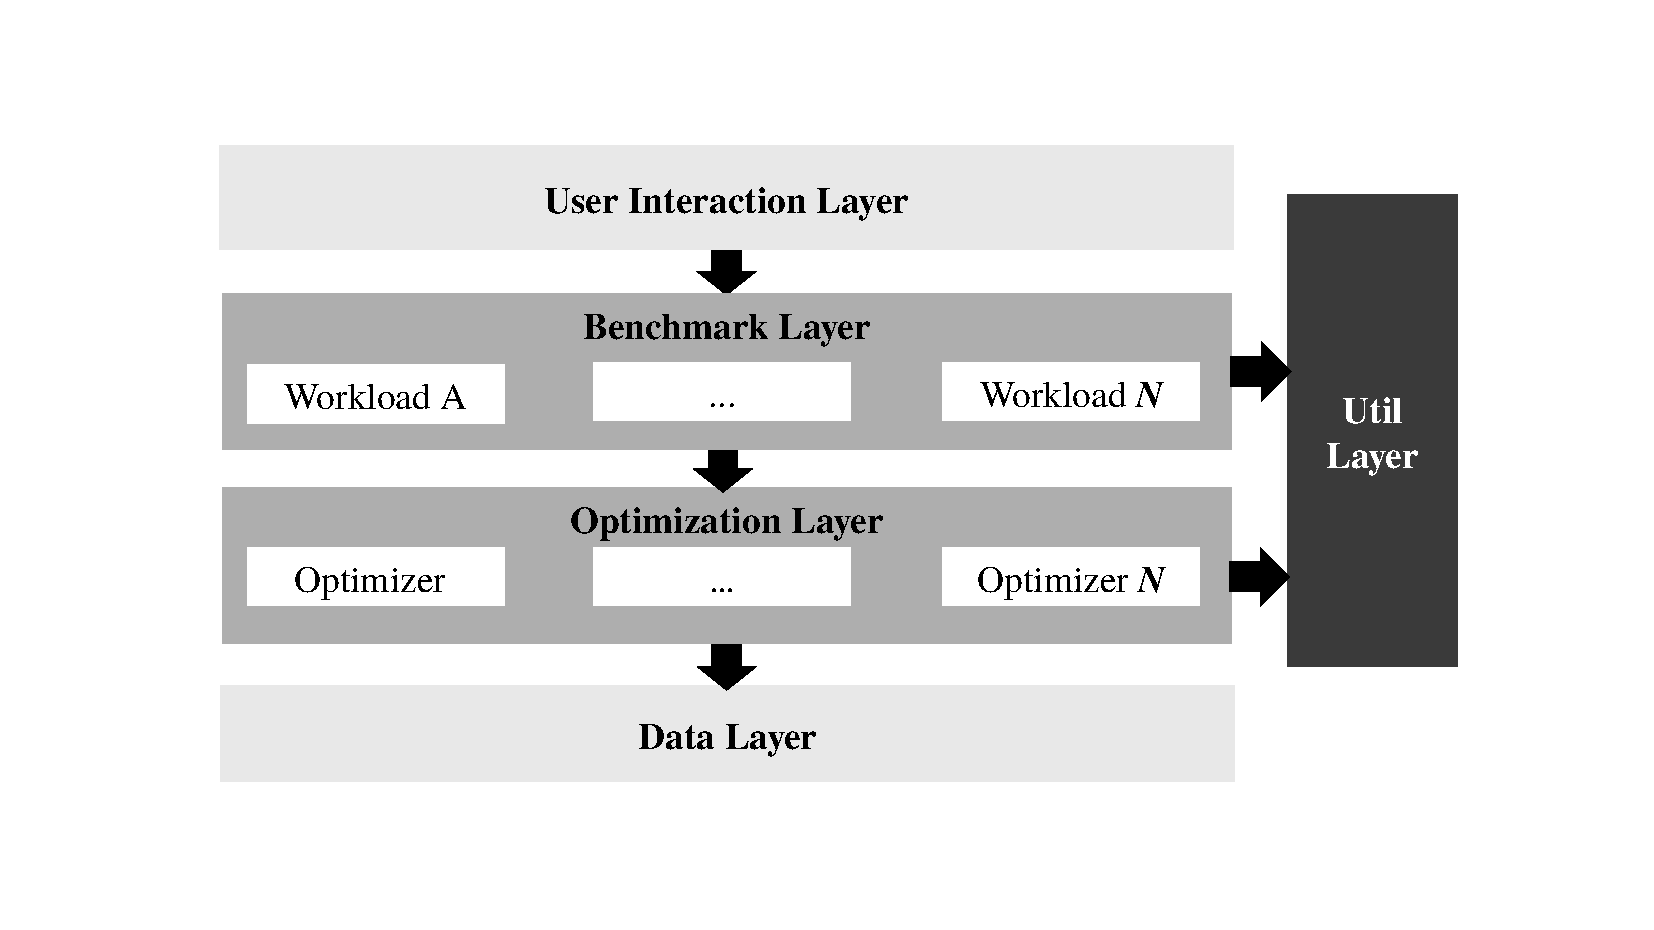
\includegraphics[width=17cm,height=10cm]{diagrams/umls/architecture-overview.pdf}
	\caption{Layered architecture of the benchmark system. The User Interaction Layer
	(implemented as a CLI) communicates with the Benchmark Layer, which manages
	multiple workloads. The Optimization Layer provides different optimizers that
	execute these workloads. All layers rely on shared functionality provided by
	the Util Layer.}
	\label{fig:architecture-overview}
\end{figure}

User interaction is handled through the command-line interface (CLI), which
allows users to configure and execute benchmark experiments. The CLI abstracts low-level
system interactions and provides a simple and consistent interface.
The Benchmark Layer is responsible for defining and managing benchmark executions.
Each workload represents a specific computational task that is executed by an optimizer.
This layer initializes workloads and provides the required configuration to the
Optimization Layer.
The Optimization Layer contains the implementations of the optimizers that execute the
workloads. These optimizers encapsulate the optimization logic and performance-critical
computations.
All layers interact with the Util Layer, which provides shared functionality such as
wrapper classes, logging mechanisms, and other cross-cutting utilities.

The following subsections describe each layer in more detail.

% ---------------------------------------------------------
\subsubsection{Benchmark Layer}
% ---------------------------------------------------------

The Benchmark Layer serves as the entry point of the application and is responsible
for defining and executing different workloads. The layer consists of two main modules:
the benchmark module and the workload module.

\begin{figure}[h]
	\centering
	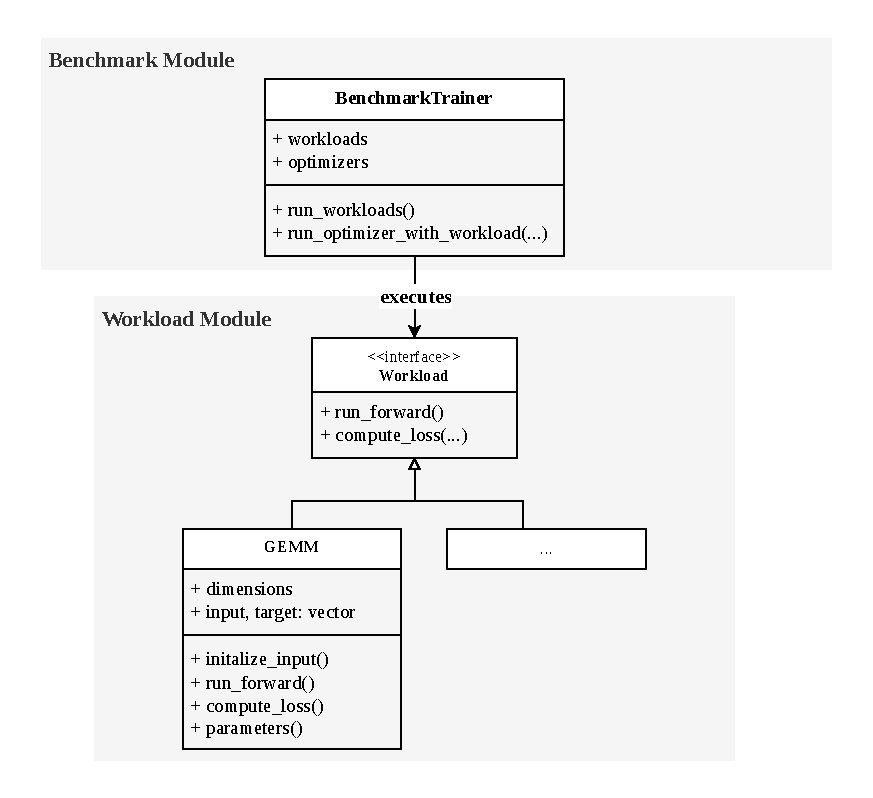
\includegraphics[width=14cm,height=14cm]{diagrams/umls/benchmark-layer-uml.pdf}
	\caption{Domain-agnostic implementation of workloads. The design enables
	maintainable integration of additional workloads in the future.}
	\label{fig:benchmark-layer}
\end{figure}

Figure \ref{fig:benchmark-layer} illustrates the implementation of the Benchmark Layer.
The class \verb|BenchmarkTrainer| is responsible for allocating the workload and
executing all required preprocessing steps before running the optimizer.
Each workload implements the abstract class or interface \verb|Workload|.
This design provides a domain-agnostic abstraction that decouples the workload
implementation from the optimization and benchmarking logic. As a result,
the benchmark program can support a wide variety of workloads.
Within the scope of this project, the class \verb|GEMM| implements a simple
neural-network workload consisting of a forward pass only. Since the current
implementation does not perform learning via backpropagation and instead only
executes forward propagation, the workload is effectively equivalent to a
general matrix multiplication (GEMM) operation rather than a full machine
learning training process.

The primary purpose of this workload is therefore to evaluate the performance
of large matrix multiplications that are transferred to and executed on the GPU
during optimization.

% ---------------------------------------------------------
\subsubsection{Optimization Layer}
% ---------------------------------------------------------

In addition to initializing workloads, the class \verb|BenchmarkTrainer|
also applies a selected optimizer to the workload.

The Optimization Layer follows a design similar to the Benchmark Layer,
allowing multiple optimizer implementations to be integrated and combined
with different workloads.

\begin{figure}[h]
	\centering
	
\includegraphics[width=14cm,height=14cm]{diagrams/umls/optimization-layer-uml.pdf}
	\caption{Domain-agnostic optimizer architecture. Different optimizer
	implementations can be provided for specific execution platforms.}
	\label{fig:optimization-layer}
\end{figure}

Figure \ref{fig:optimization-layer} shows the implementation concept of the
Optimization Layer. Each optimizer implements the abstract class or interface
\verb|Optimizer|.
All optimizer implementations must provide an implementation of the
\verb|step| function. This function is executed during each iteration of the
training or optimization process and updates the parameters toward a local
or global optimum.
For example, the Adam optimizer is implemented in the classes
\verb|AdamOptimizer|, \verb|AdamOptimizerCl| (OpenCL), and
\verb|AdamOptimizerCu| (CUDA). In this case, the \verb|step| function performs
a parameter update in the parameter space at time step $t$, as described by
Kingma and Ba \cite{adam}.
Because data transfer to GPU devices differs between frameworks,
additional functions such as \verb|fromDevice| or
\verb|launch_adam_kernel| are required to manage device-specific execution.

% ---------------------------------------------------------
\subsubsection{Util Layer}
% ---------------------------------------------------------

The Util Layer provides shared functionality that is used throughout the
entire project. These utilities address cross-cutting concerns such as
data representation, logging, and framework abstraction.

\begin{figure}[h]
	\centering
	
\includegraphics[width=14cm,height=14cm]{diagrams/umls/util-layer.pdf}
	\caption{Utility layer components providing shared functionality
	across the application.}
	\label{fig:util-layer}
\end{figure}

Figure \ref{fig:util-layer} illustrates the interactions between the
different utility components. Data view classes such as
\verb|HostParamsView| and \verb|DeviceParamView| provide platform-specific
representations of parameter data.
Since OpenCL and CUDA require different data representations for GPU
execution, parameter data must be converted from the host representation
(\verb|HostParamsView|) to the device representation
(\verb|DeviceParamView|). This conversion is handled by the respective
optimizer implementations.
Furthermore, optimizer classes interact with wrapper classes that
encapsulate OpenCL and CUDA functionality. These wrappers significantly
reduce the amount of boilerplate code required to execute workloads on
GPU devices.
At the end of each benchmark execution, the collected benchmark results,
stored in the \verb|benchmarkData| class, are written to a CSV file.
This process is handled by the \verb|Logger| class.

% ---------------------------------------------------------
\subsubsection{Data Layer}
% ---------------------------------------------------------

The Data Layer consists of the benchmark CSV file that stores the results
of all benchmark executions. These results can later be used for further
analysis.
A snippet of the file is shown in Listing \ref{listing:benchmark-data}.

\begin{verbatim}
timestamp,framework,workload_name,workload_type,device,batch_size,input_size,optimizer,learning_rate,beta1,beta2,epsilon,time_ms,batch_index,loss
2026-02-02-11-13-36,None,GEMM_Adam_CPU,compute,CPU,10,1048723456,Adam,0.001,0.9,0.999,1e-08,113,1,0
2026-02-02-11-13-41,None,GEMM_Adam_CPU,compute,CPU,10,1048723456,Adam,0.001,0.9,0.999,1e-08,83,2,0.0224746
...
\end{verbatim}

The goal of the logging system is to capture as much contextual information
as possible from each benchmark execution. Most of the recorded data
describes the experimental configuration, including hyperparameters such as
\verb|learning_rate|, \verb|beta1|, and \verb|beta2|.
The actual performance measurement is represented by the variable
\verb|time_ms|. However, including the surrounding context allows a more
detailed analysis of potential correlations between execution conditions
and performance characteristics.


\pagebreak
\section{Benchmark results}
% What are the results?
% TODO increase workload sizes so we can compare really large workloads
% TODO build time in OpenCL

\subsection{Results for NVIDIA GeForce GTX 970}
The benchmark program using the Adam optimizer and the \ac{GEMM} workload was first executed
on an NVIDIA GeForce GTX 970 with 8 GB of VRAM. For this benchmark, the following results
were obtained for data transfer time and computation time using CUDA and OpenCL.

\begin{table}[th]
	\caption{Data transfer time and computation time across all batch indices}
	\label{tab:gtx970results}
	\centering
	\begin{NiceTabular}{lrrr}
		\CodeBefore
		\rowcolors{2}{gray!10}{white}
		\Body
		\textbf{Metric} & \textbf{CUDA} & \textbf{OpenCL} & \textbf{Perf. Ratio} \\
		Average data-transfer time (ms) & 4.06 & 4.43 & ? \% \\
		Average computation time (ms) & 2.45 & 0.77 & ? \% \\
	\end{NiceTabular}
\end{table}

Table \ref{tab:gtx970results} presents the benchmark results obtained with the specified
hyperparameters. The data transfer time was averaged across all measurements performed for
both OpenCL and CUDA. The results show that CUDA is 9\% faster in terms of data transfer time
on the NVIDIA GeForce GTX 970. Similarly, the computation time was averaged over all runs,
resulting in CUDA being 66\% faster than OpenCL.

\begin{figure}[th]
	\begin{center}
		\includegraphics[width=16cm, height=8cm]{nvidia_geforce_gtx_970_compute_and_transfer_batch_line_normalized}
	\end{center}
	\caption{Results of running the GEMM workload using the Adam optimizer}
	\label{fig:pltgtx970}
	\centering
\end{figure}

Figure \ref{fig:pltgtx970} shows the average computation time per \verb|batch_index| and
also includes the average loss per \verb|batch_index| for both frameworks. This illustrates
the efficiency of both frameworks while also providing an indication of their reliability.
The figure shows that the loss decreases over time, which matches the expected behavior
during optimization. Furthermore, the figure highlights the results summarized in
Table \ref{tab:gtx970results}. This data shows that on data transfer time CUDA provides 
better results while for computation OpenCL provides better results on the GTX 970 representing
here the Maxwell architecture from NVIDIA.

\subsection{Results for RTX 5000}
\subsection{Results for A-100}

\section{Discussion}
% Summary of results
	
	% --- references ---
	
	\newpage
	\printbibliography[heading=bibintoc]
	
\end{document}
